Das verwendete System hat folgende Spezifikationen: Intel(R) Core(TM) i7-10710U
CPU, 1.10 GHz, 16 GB Arbeitsspeicher, Ubuntu 22.04.2 LTS, 64 Bit.
Linux Kernel 5.19.0-45-generic.
Kompiliert wurde mit GCC 11.3.0 mit der Option \texttt{-O2}.
\\
Performance-Tests werden für V0 (die Implementierung mit Vektoroptimierung)
und V1 (die Implementierung mit Wrapper-Funktionen für String-Operationen) durchgeführt.

\subsection{Laufzeit-Tests}
Wir verglichen die Laufzeit für Operationen zwischen Dateien mit unterschiedlichen Datenmengen,
 unterschiedlicher Entropie (Inhaltswiederholung), Datenlängen, die
(nicht) ganzzahlige Vielfache von 16 sind und Dateien mit redundanten 
Datenlängen von 1 oder 15 usw.

\subsubsection{Voraussetzungen für die Laufzeit-Tests}
Wir gestalteten unsere Tests so, dass Sie die in der Vorlesung genannten 
Voraussetzungen \cite{benchmarking} erfüllen: 
\begin{itemize}
    \item Um die Genauigkeit der Ergebnisse zu garantieren, wurde jeder Test 250.000
          Mal wiederholt, so dass die Gesamtlaufzeit 1 Sekunde betrug.
    \item Aufgrund der Varianz der Zeittests führen wird derselben Test
          mindestens dreimal durchgeführt und der Durchschnitt berechnet.
    \item Die Tests wurden auf einem Personal Computer durchgeführt, da stärkere 
         Varianzen beim Testen in der \texttt{lxhalle} über \texttt{ssh} beobachtet wurden. 
    \item Der Computer sollte sich nicht im Energiespar-Modus befinden \cite{energySaving}, sonst
          verlängert sich die Laufzeit und die Varianz der Ergebnisse nimmt zu.
    \item Die Optimierungsstufe sollte mindestens \texttt{-O2} sein. 
    \item Es werden \texttt{clock\_gettime} als funktion und \texttt{CLOCK\_MONOTONIC} als Uhr
          gewählt, da sie präziser sind als andere Funktionen.  
\end{itemize}
  
Die Zeittests erfordern ein sehr hohes Niveau an Genauigkeit und Präzision, \cite{energySaving}
andernfalls sind die Ergebnisse gegenstandslos bzw. unwissenschaftlich.

\subsubsection{Ergebnisse der zeitbasierten Tests}
Der Unterschied in der Laufzeit zwischen $V0$ und $V1$ ist unter \texttt{O2} nicht signifikant,
testet man allerdings in \texttt{O0} ist $V0$ deutlich besser als $V1$.
Aufgrund der Voraussetzungen konzentrieren
wir uns in diesem Abschnitt jedoch auf die Ergebnisse in \texttt{O2}.
Auf Grundlage der Ergebnisse der Laufzeittests und \ref*{img:test1} kommen wir zu folgenden Entschlüssen:
\begin{itemize}
    \item [(a)] \textbf{Die Laufzeit ist proportional zur Dateigröße.}
          \\
          Die verbrauchte Zeit steigt mit steigender Dateigröße linear an.
    \item [(b)] \textbf{Mittels loop-unrolling kann die Laufzeit reduziert werden}\cite{gnuOptimierung}
          \\
          Fügt man die Option \texttt{-funroll-loops} in die Makefile ein, kann man 
          einen klaren Speedup erkennen.

    \item [(c)] \textbf{Kein Zusammenhang zwischen SIMD und verbrauchter Zeit}
          \\
          Im MD2-Hash-Algorithmus umfassen die Berechnung der Prüfsumme und die 
          Generierung des Hash-Wertes mehrere Schritte. Einer dieser Schritte 
          ist die Byte-Substitution, die mehrmals auf dem Eingabe-String durchgeführt wird.
          Dieser Prozess erfolgt sequenziell und behandelt jedes Byte einzeln. 
          Die Substitution basiert sowohl auf dem aktuellen Byte-Wert, der 
          verarbeitet wird, als auch auf dem Ergebnis, das aus dem vorherigen 
          Substitutionsschritt erzielt wurde und ist somit iterativ in der Natur.
          Eine Vektorisierung mittels SIMD oder Multithreading erweist sich deswegen als kaum effektiv.
\end{itemize}

          \begin{figure}[H]
            \label{img:test1}
                  \centering
                  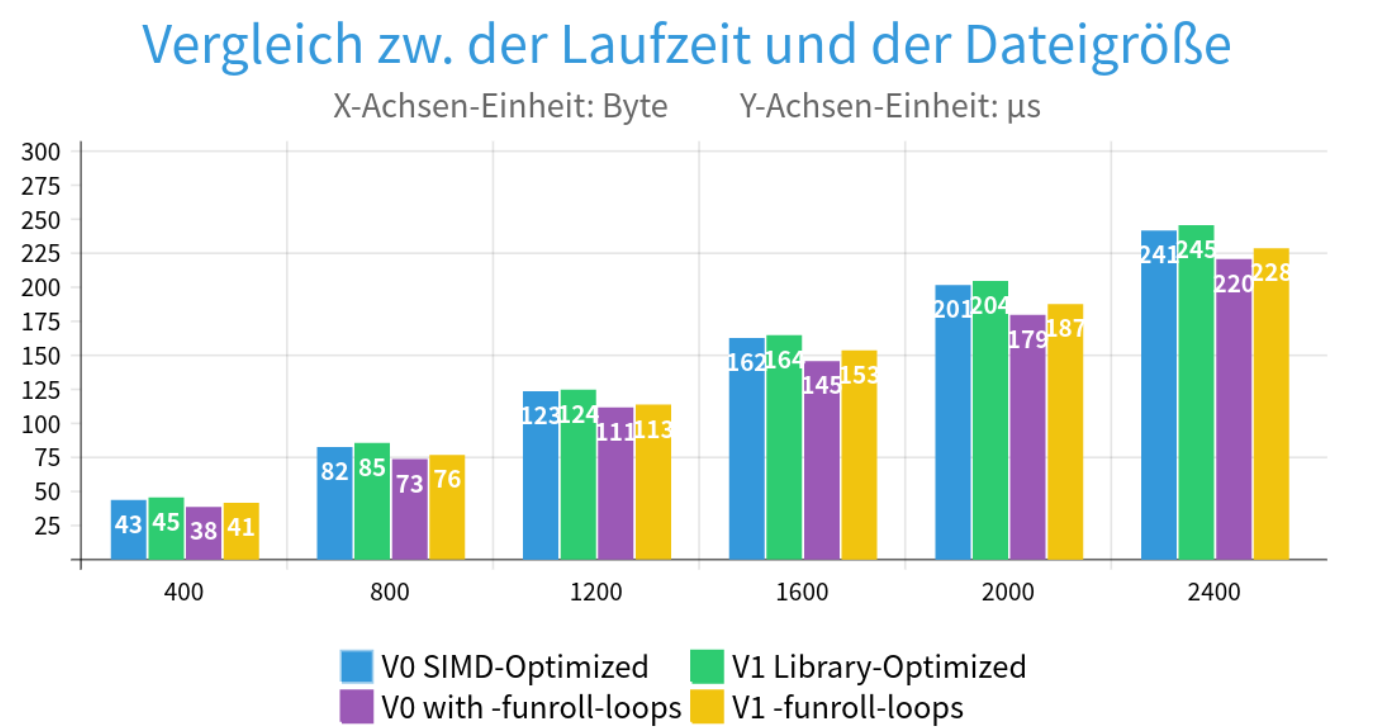
\includegraphics[height=6cm, width=10cm]{pics/4laufzeit.png}
                  \caption{Vergleich zwischen Laufzeit und Dateigröße.
                    Die Berechnungen wurden mit Eingabgrößen von 400 bis 2400 Bytes jeweils 250000 mal
                    durchgeführt und das arithmetische Mittel für jede Eingabegröße auf der $y$ Achse eingetragen.
                    }
              \noindent
          \end{figure}


\subsection{Tests zur Programmgröße}
Bei der Untersuchung Operationenanzahl (Menge des Codes) stellten wir fest,
dass $V0$ deutlich weniger Operationen benötigt als $V1$.
\\
Die .c-Dateien zeigen, dass die Implementierung mit Intrinsics die beste ist.
Darüber hinaus wurde der Assembly-Code der verschiedenen Implementierungen mit dem Terminalbefehl
\texttt{objdump -d -M intel main | less} überprüft. \cite{analyseDesKompiliertenProgramms}.

\begin{figure}[H]
        \centering
        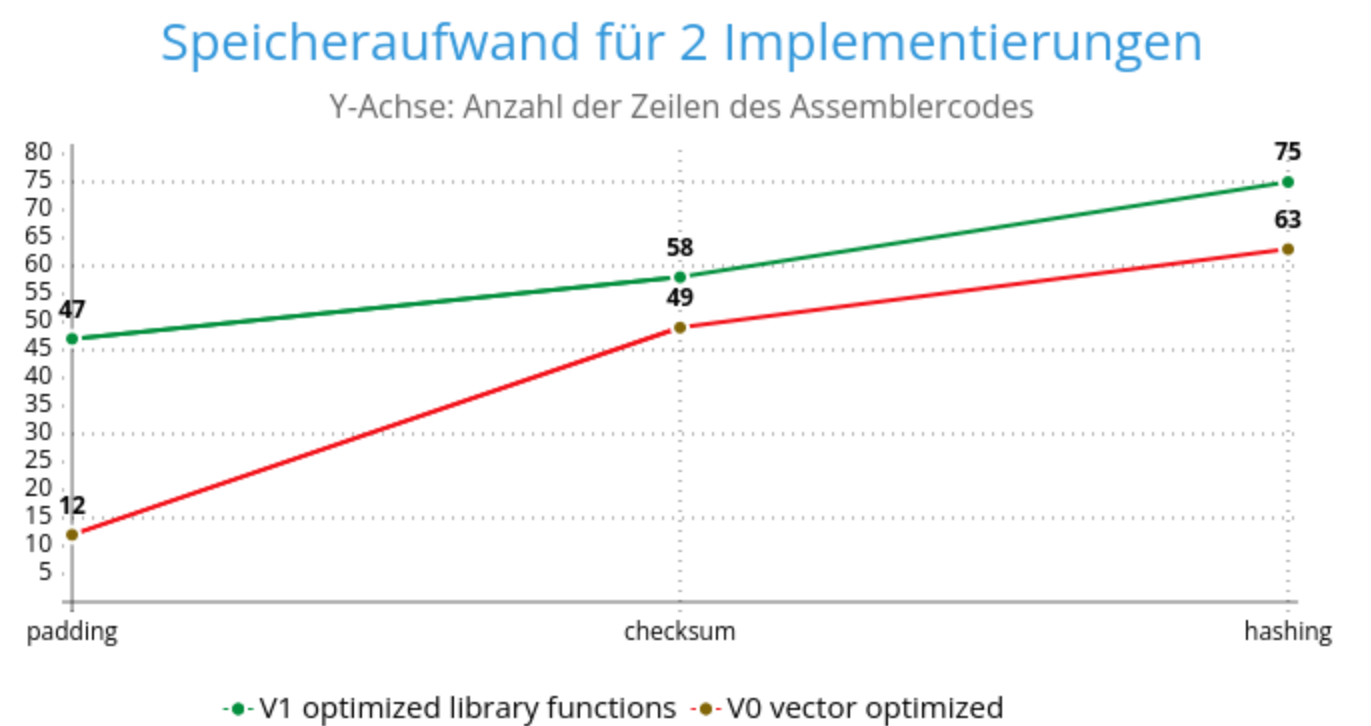
\includegraphics[height=6cm, width=10cm]{pics/SpeicherAufwand.png}
        \caption{Speicheraufwand von $V0$ und $V1$}
        \label{img:test2}
    \noindent
\end{figure}

Der auf V0 basierende Assembly-Code hat viel weniger Vergleichs -und Sprungoperationen.
Außerdem wurde in $V0$ die xmm-Erweiterung eingeführt, welche die Anzahl der Instruktionen
weiter reduziert (vgl. \ref{img:test2}).
\\
Wird die Option \texttt{-funroll-loops} verwendet, wird der entstehende Code
größer und weniger lesbar (vgl. \ref{img:test3}).

\begin{figure}[H]
        \centering
        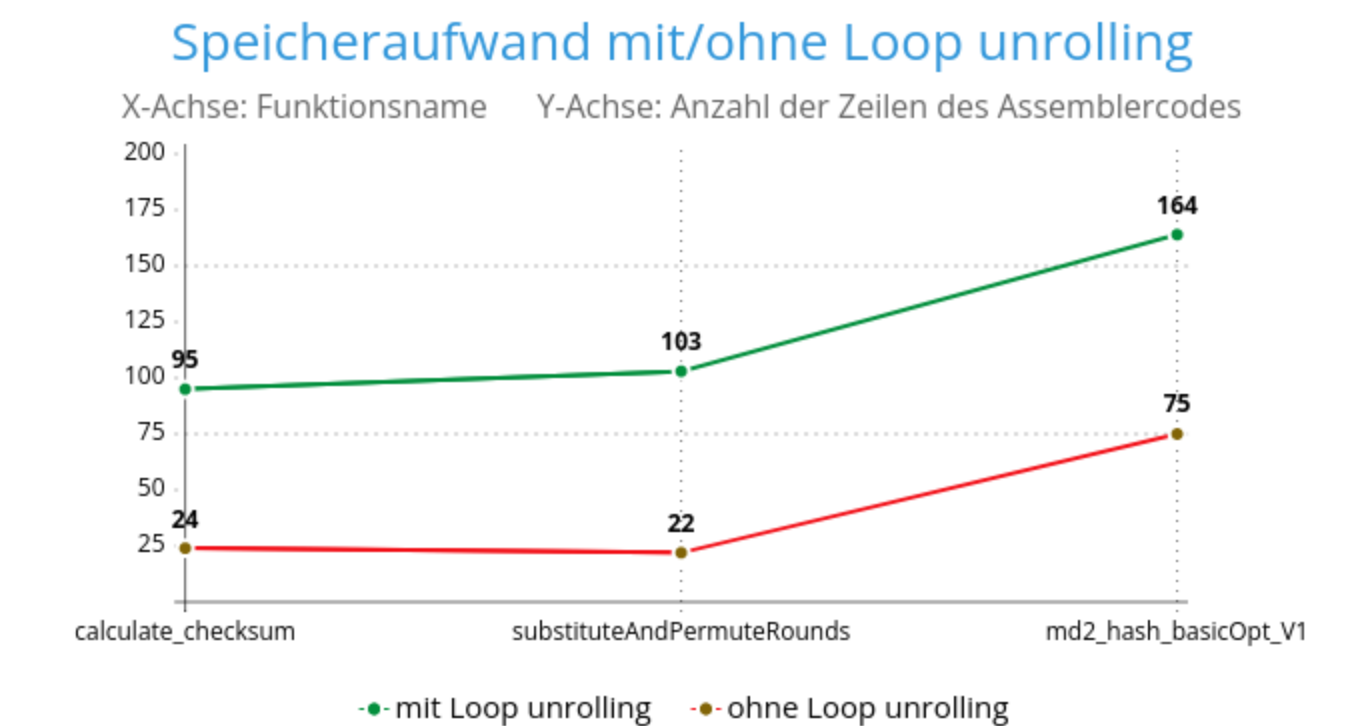
\includegraphics[height=6cm, width=10cm]{pics/loopUnrolling.png}
        \caption{Speicheraufwand mit bzw. ohne Loop unrolling}
        \label{img:test3}
    \noindent
\end{figure}

Loop-Unrolling kann die Laufzeit des Programms reduzieren, kommt aber auf kosten von
Lesbarkeit und die Speicher.

%Lack of detail. Need to elaborate further
%\subsection{Andere Optimierungen}
%Wir nahmen zudem weitere, kleinere Optimierungen an unserer Implementierung vor.
%\\
%Ursprünglich basierte die Logik auf \texttt{if}-Anweisungen oder \text{switch}-Anweisungen.
%\\
%Danach haben wir unsere Codelogik optimiert, um sie weniger redundant zu machen.
%Wie in der Vorlesung erwähnt\cite{gnuOptimierung}, können fortgeschrittenere Algorithmen zur
%Optimierung verwendet werden.
%\\
%Anschließend haben wir die GCC-Wrapper-Funktionen verwendet, um unsere Implementierung
%weiter zu optimieren.
%Darüber hinaus haben wir auch manuelle Schleifenvertauschungen und
%Schleifenerweiterungen ausprobiert.
%\\
%Allerdings zeigten sie nicht den gewünschten Optimierungseffekt oder sogar eine
%Verschlechterung.

\subsection{Zusammenfassung der Performanzanalyse}
Die Implementierung mit Intrinsics ist am effizientesten.
Die Verwendung von Loop Unrolling führt zu einem deutlichen Geschwindigkeitszuwachs,
die Codegröße steigt damit aber auch an.
%\\
%Man könnte sich für weitere Verbesserungen tiefer mit Multithreading auseinandersetzen.
%Die Codegröße dieses Projekts ist nicht groß genug, um eine signifikante Optimierung
%der Laufzeit unter $O2$ zu erreichen, aber aus Sicht der Codegröße schon.
\\
MD2 ist ein byteorientierter Hash-Algorithmus.\cite{rfc1319}
In der Tat verarbeiten alle Instruktionen 8-Bit Blöcke.
Dies verbessert zwar die Kompatibilität mit älteren Architekturen und vereinfacht die
Implementierung, führt aber auch
zu der schlechten Performanz und Optimierbarkeit des MD2-Algorithmus.
\\
Heutige Prozessoren können (mindestens) 32-Bit-Datenwörter verarbeiten, woran sich alle
modernen Hashfunktionen orienteren, z.B. MD4, MD5, die Familien RIPEMD
und SHA.
Daher schränkt die Logik des Algorithmus allein die Optimierungsmöglichkeiten ein.